\documentclass{article}
\usepackage[utf8]{inputenc}
\usepackage{subfig}

%References
\usepackage{natbib}
%IMPORTANT use https://www.citationmachine.net/ if you need to generate references!
% \citep{reference} creates Harvard Style references throughout

%Colors
\usepackage{xcolor}

\usepackage[protrusion=true,expansion]{microtype}

%Code Markup
\usepackage[outputdir=cache]{minted}
%Syntax Highlighting Style
\definecolor{bggray}{RGB}{40,40,40}
%Macro to make a Syntax Highlighter For Java files 
%Use \javacode{filename.java} to insert a Java File W/ Syntax Highlighting file into the PDF
\newmintedfile[javacode]{java}{
	style=fruity,
	bgcolor=bggray,
	linenos,
	breaklines,
	tabsize=2,
	obeytabs
}

\newmintedfile[bashoutput]{txt}{
	style=fruity,
	bgcolor=lightgray,
	breaklines,
	tabsize=2,
	obeytabs
}

%Page Margins and stuff
\usepackage{geometry}
 \geometry{
 a4paper,
 total={170mm,257mm},
 left=20mm,
 }

%Pictures
\usepackage{graphicx}
\graphicspath{ {./images/} }

%Move the title position
\usepackage{titling}

\setlength{\droptitle}{-8.5em} %Up, near the top but not too high
%Section Heading formatting
\usepackage{titlesec}
\titleformat{\section}
  {\normalfont\Large\bfseries}{\thesection}{1em}{}[{\titlerule[0.8pt]}]

\title{Assingment 3 - Programming Paragidms }
\author{Daniel Hannon (19484286)}
\date{Novemeber 2021}

\begin{document}
	\maketitle
	\section{Question 1}
	\inputminted{prolog}{question1.pl}
	\begin{figure}[h!]
		\centering
		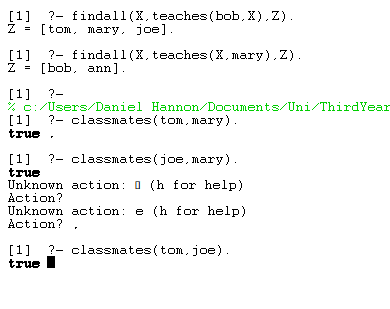
\includegraphics[width=0.6\textwidth]{question1.png}
	\end{figure}
	1.4 returns false as they are both students so neither instructs and as a result ann definitely does not teach joe.
	\newpage
	\section{Question 2}
	\inputminted{prolog}{question2.pl}
	\begin{figure}[h!]
		\centering
		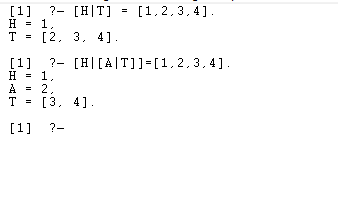
\includegraphics[width=0.6\textwidth]{question2_1.png}
	\end{figure}
	\begin{figure}[h!]
		\centering
		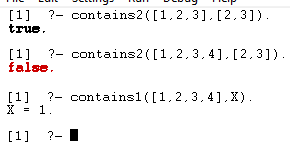
\includegraphics[width=0.6\textwidth]{question2_2.png}
	\end{figure}
	\newpage
	\section{Question 3}
	\inputminted{prolog}{question3.pl}
	\begin{figure}[h!]
		\centering
		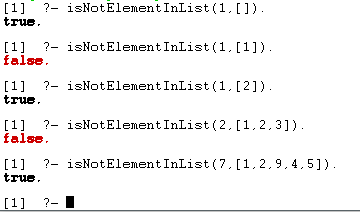
\includegraphics[width=0.6\textwidth]{question3.png}
	\end{figure}
	\section{Question 4}
	\inputminted{prolog}{question4.pl}
	\begin{figure}[h!]
		\centering
		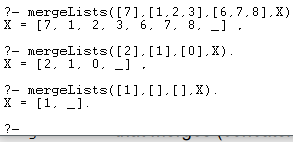
\includegraphics[width=0.6\textwidth]{question4.png}
	\end{figure}
	\newpage
	\section{Question 5}
	\inputminted{prolog}{question5.pl}
	\begin{figure}[h!]
		\centering
		
\includegraphics[width=0.6\textwidth]{question5.png}
	\end{figure}
	\section{Question 6}
	\inputminted{prolog}{question6.pl}
	\begin{figure}[h!]
		\centering
		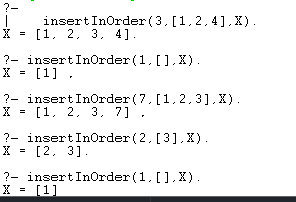
\includegraphics[width=0.6\textwidth]{question6.png}
	\end{figure}
	%Sets to Harvard Style and links the references file
	\bibliographystyle{agsm}
	\bibliography{references}
\end{document}